
\documentclass{beamer}
\usepackage{tikz}
\usepackage{multicol}
\usepackage{tikzsymbols}
\usepackage{wasysym}
\usepackage{mathpazo}
\usepackage{amsmath}
\usepackage{graphicx}
\usepackage{quotmark}
\usepackage{listings}
\usepackage[nodayofweek]{datetime}
\usepackage{showexpl}
\usepackage[T1]{fontenc}
\usepackage{framed}
\usepackage[utf8]{inputenc}
\usepackage[absolute,overlay]{textpos}
\date{\today}
\lstdefinestyle{basic}{
    captionpos=t,%
    basicstyle=\footnotesize\ttfamily,%
    numberstyle=\tiny,%
    numbers=left,%
    stepnumber=1,%
    frame=single,%
    showspaces=false,%
    showstringspaces=false,%
    showtabs=false,%
    %
    keywordstyle=\color{blue},%
    identifierstyle=,%
    commentstyle=\color{gray},%
    stringstyle=\color{magenta}%
}
\usetheme{Ilmenau}
\setbeamertemplate{navigation symbols}{}
\setbeamertemplate{caption}[numbered]
\usefonttheme{serif}
\usefonttheme{professionalfonts}
\geometry{paperwidth=600px,paperheight=400px}
\pgfdeclareimage[height=.2\textheight]{eel}{EEL-logo}
\graphicspath{{images/}}

\begin{document}





\setbeamertemplate{footline}{\leavevmode\hbox{\begin{beamercolorbox}[wd=.4\paperwidth,ht=2.25ex,dp=1ex,center]{author in head/foot}\usebeamerfont{author in head/foot}\insertshortauthor\end{beamercolorbox}\begin{beamercolorbox}[wd=.6\paperwidth,ht=2.25ex,dp=1ex]{title in head/foot}\usebeamerfont{title in head/foot}\hskip 2mm\insertshorttitle\hfill\insertframenumber{} / \inserttotalframenumber\hspace*{1ex}\end{beamercolorbox}}\vskip0pt}

\setlength{\TPHorizModule}{\textwidth}
\setlength{\TPVertModule}{\textwidth}

\lstset{explpreset={},	hsep=6mm,	breaklines=true,	language=[LaTeX]TeX,	postbreak=\raisebox{0ex}[0ex][0ex]{\ensuremath{\hookrightarrow\space}},	basicstyle=\small\ttfamily,	keywordstyle=\color{blue},	commentstyle=\color{green!60!black},	frame=single,	numbers=left,	numberstyle=\tiny,	}

\title{Creating documents in \LaTeX{} --- a basic tutorial}
\author{Luiz T. F. Eleno}
\institute[EEL--USP]{Departamento de Engenharia de Materiais\\Escola de Engenharia de Lorena\\Universidade de São Paulo (EEL--USP)\\Lorena (SP), Brazil\\[2mm] 
\includegraphics[width=25mm]{EEL-logo}}
\newdate{apres}{18}{10}{2018}
\date{Lorena, \displaydate{apres}}

\frame{\titlepage}

\frame{\frametitle{Contents}\begin{multicols}{2}\tableofcontents\end{multicols}}

\let\orilabel\label


\section{Preliminaries}




\subsection{in the form of a prelude}



\begin{frame}
 \frametitle{What is \LaTeX}
  


\centering

{\Huge \LaTeX{} --- A document preparation system}


\vspace{ 5mm }


\begin{itemize}
  \item \LaTeX{} is a \emph{markup} language that allows you to write documents focusing on contents instead of formatting
  \item You don't have to worry about fonts or section/figures/tables/citation numbering
\begin{itemize}
  \item \LaTeX{} will do it automatically for you
\end{itemize}
  \item All formatting will be taken care of by \emph{packages}, or libraries you can load at the beginning of the document
  \item $\Rightarrow$ you can then focus on your text, which is the most important part of your document, leaving all the ``makeup'' to \LaTeX
\end{itemize}

\begin{itemize}
  \item \LaTeX{} follows the WYMIWYG (\emph{What you MEAN is what you get}) concept
\begin{itemize}
  \item instead of the WYSIWYG (\emph{what you SEE is what you get}) concept used by most word processors
\begin{itemize}
  \item which, usually, are more like WYSIWYTYG (\emph{what you see is what you THINK you get\ldots})
\end{itemize}
\end{itemize}
\end{itemize}


\vspace{ 5mm }


\Springtree[10] \quad \Summertree[10] \quad \Autumntree[10] \quad \Wintertree[10]\\
{\tiny (trees generated using the \texttt{tikzsymbols} package)}

  
\end{frame}
\begin{frame}
 \frametitle{Distributions}
  


\begin{itemize}
  \item In order to run \LaTeX{} in your computer, you need a \LaTeX{} \emph{distribution}
\begin{itemize}
  \item There are several options; the two given below are the most widespread
\end{itemize}
\end{itemize}

\begin{block}{Selected \LaTeX{} distributions:}
\begin{itemize}
  \item TeXLive (linux) --- \url{https://www.tug.org/texlive} \\ 
\includegraphics[ height=20mm]{texlive}
  \item MikTeX (windows) --- \url{https://miktex.org} \\ 
\includegraphics[ height=20mm]{miktex}
\end{itemize}
\end{block}

\begin{itemize}
  \item All popular Linux distributions (ubuntu, arch, opensuse, fedora, mandriva, etc.) have preset \LaTeX{} platforms in their repositories
  \item Mik\TeX{} is also very easily installed on windows
\end{itemize}

\begin{itemize}
  \item There are also, nowadays, online \LaTeX{} platforms that you can use without download or install
\begin{itemize}
  \item but a very fast internet connection is recommended to avoid frustration and annoyance
\end{itemize}
\end{itemize}

\begin{itemize}
  \item The distributions listed above are free and open source
\end{itemize}

  
\end{frame}
\begin{frame}
 \frametitle{Editors}
  


\begin{itemize}
  \item A \LaTeX{} IDE (integrated development environment) is highly recommended, especially for newbies
\end{itemize}

\begin{block}{Selected \LaTeX{} IDEs:}

\begin{columns}

\column{.5\textwidth}

\begin{itemize}
  \item TeXStudio --- \url{https://www.texstudio.org} \\ 
\includegraphics[ height=20mm]{texstudio}
  \item TeXMaker --- \url{http://www.xm1math.net/texmaker} \\ 
\includegraphics[ height=20mm]{texmaker}
  \item TeXWorks --- \url{http://www.tug.org/texworks} \\ 
\includegraphics[ height=20mm]{texworks}
\end{itemize}

\column{.5\textwidth}

\begin{itemize}
  \item LyX --- \url{https://www.lyx.org} \\ 
\includegraphics[ height=20mm]{lyx}
  \item Authorea (online) --- \url{https://www.authorea.com} \\ 
\includegraphics[ height=20mm]{authorea}
  \item Overleaf (online) --- \url{https://www.overleaf.com} \\ 
\includegraphics[ height=20mm]{overleaf}
\end{itemize}

\end{columns}

\end{block}

\begin{itemize}
  \item To use any of them, you MUST first install a \LaTeX{} distribution
\begin{itemize}
  \item except the online IDEs, of course
\end{itemize}
  \item All editors listed above are free; some are also open source
\end{itemize}

  
\end{frame}

\section[Structure]{Structure}




\subsection{About the organization of a \LaTeX{} document}



\begin{frame}[containsverbatim]
 \frametitle{Preamble and body}
  


\begin{itemize}
  \item A typical \LaTeX{} document: a file with \texttt{.tex} extension
  \item it has two major parts: a \emph{preamble} and a \emph{body}
\end{itemize}
\begin{lstlisting}
\documentclass[options]{class type}

% This is the document PREAMBLE
% here go configuration packages and commands

% all LaTeX commands start with a \ (backslash)
% everything following a % is a comment
% you can insert comments anywhere in the document
% if you want a % to appear in your text, escape it using \%

% the document class is always the first line of your document
% you can define some options that affect the formatting of the chosen class type
% some class types: article, book, report
% common options: 10pt|11pt|12pt (font size), oneside|twoside (use one or both sides of the paper)

\begin{document}

% This is the body of your document
% Your text, tables, figures, etc. (generically, your content) go here

\end{document}

\end{lstlisting}

  
\end{frame}
\begin{frame}[containsverbatim]
 \frametitle{Packages}
  


\begin{itemize}
  \item In the preamble are loaded packages (libraries) that affect and provide new commands
\begin{itemize}
  \item for instance, font packages, math packages, bibliography packages, etc.
\end{itemize}
  \item Packages are loaded with the command \lstinline!\usepackage[options]{package name}!
\end{itemize}

\begin{block}{A few useful examples:}

\begin{itemize}
  \item \lstinline!\usepackage[a4paper, margin=20mm]{geometry}! loads the \texttt{geometry} package and sets the paper size to A4 and all margins to 20\,mm
  \item \lstinline!\usepackage[utf8]{inputenc}! allows you to use accented characters (á, ã, ã, ä, ç, etc)
\begin{itemize}
  \item the option used (\texttt{utf8}) is for files set up with the unicode encoding (other encodings are also possible)
  \item newest versions of \LaTeX{} are automatically set up for \texttt{utf8} encoding (i.e., there is no need to call this package anymore)
\end{itemize}
  \item \lstinline!\usepackage{setspace}! gives access to interline spacing
\begin{itemize}
  \item after loading the package, set the spacing used in the document with one of the following commands:
\begin{enumerate}
  \item \verb!\singlespacing! (default)
  \item \verb!\onehalfspacing!
  \item \verb!\doublespacing!
\end{enumerate}
\end{itemize}
  \item \lstinline!\usepackage{graphicx}! permits the inclusion of figures (jpg, png, eps, pdf, etc.) in the document
\end{itemize}

\end{block}

  
\end{frame}
\begin{frame}[containsverbatim]
 \frametitle{Non-english languages}
  


\begin{itemize}
  \item \LaTeX{} automatically hyphenates your words
  \item Also, a few words (like chapter, section, page, etc.) and formatted date are sometimes used
\begin{itemize}
  \item but the default language is American English
\end{itemize}
  \item To change the language of the document, call the \texttt{babel} package in the preamble
\end{itemize}

% to use non-ascii characters in the UTF-8 encoding, if your language requires them
% \usepackage[utf8]{inputenc}

\begin{lstlisting}
% to hyphenate and translate keywords to brazilian portuguese (for instance)
\usepackage[brazil]{babel}

\end{lstlisting}

  
\end{frame}
\begin{frame}[containsverbatim]
 \frametitle{Multi-file documents}
  


\begin{itemize}
  \item Your document can be spread through multiple files
  \item The master document calls other files with the \verb!\input! command:
\end{itemize}

\begin{lstlisting}
\documentclass[12pt]{article}

% preamble

\input{style.tex} % all packages and configuration commands

\begin{document}

% body

\input{chapter1.tex}

\input{chapter2.tex}

\end{document}

\end{lstlisting}

  
\end{frame}

\section{Sectioning}




\subsection{How to partition a \LaTeX{} document}



\begin{frame}[containsverbatim]
 \frametitle{Document title}
  


\begin{itemize}
  \item The title of your document comes from the following commands:
\end{itemize}
\begin{lstlisting}
\title{My article}
\author{My name}
\date{time I wrote it} % if not given, results in the \today command's output

\maketitle % format and prints the title for you
% optionally, include titlepage among the \documentclass options for a title cover
\end{lstlisting}

\institute{}
\date{\today}

\begin{itemize}
  \item If you're using the \texttt{beamer} class (as I'm doing right now), you'll get something like this:
\end{itemize}

\begin{LTXexample}
\title{A wonderful talk}
\author{presented by myself}

\maketitle
\end{LTXexample}

\begin{itemize}
  \item \texttt{title}, \texttt{author} and \texttt{date} can be either in the preamble or in the body of the document
  \item \texttt{maketitle} must be issued from within the body of the document
\end{itemize}

  
\end{frame}
\begin{frame}[containsverbatim]
 \frametitle{Chapters, sections and subsections}
  


\begin{itemize}
  \item Creating headings in your document is straightforward:
\end{itemize}

\begin{lstlisting}
\chapter{My chapter} % beware: the article class has no chapters!
\label{cha:mycha}

\section{A section}
\label{sec:mysec}

\subsection{A sub-section}
\label{sub:mysubsec}

\subsubsection{A sub-sub-section}
\label{ssub:mysubsubsec}
% And that's enough for most purposes!
% If you really need more, there are packages that allow you to add more sublevels
\end{lstlisting}

\begin{itemize}
  \item We'll soon learn what is the purpose of the several \verb!\label! commands
\begin{itemize}
  \item they are optional and, for now, see them simply as tags to identify each heading
\end{itemize}
\end{itemize}

  
\end{frame}
\begin{frame}[containsverbatim]
 \frametitle{Tables of contents}
  


\begin{itemize}
  \item You can add tables of contents and  lists of tables and figures:
\end{itemize}

\begin{lstlisting}
\tableofcontents

\listoffigures

\listoftables
\end{lstlisting}

\begin{itemize}
  \item (Soon we'll see how to insert figures and tables to be shown in the lists above!)
\end{itemize}

  
\end{frame}

\section{Formatting}




\subsection{Changing appearances}



\begin{frame}[containsverbatim]
 \frametitle{Typesetting a \LaTeX{} document}
  


\begin{itemize}
  \item Basic typesetting:
\begin{itemize}
  \item any amount of space between characters will be shortened to just one space character
\begin{itemize}
  \item use \textasciitilde{} to add space (and \verb!\textasciitilde{}! if you want the \textasciitilde{} character)
\end{itemize}
\end{itemize}
  \item leave any amount of blank lines to start a new paragraph
\end{itemize}

\begin{LTXexample}
This is a paragraph.

And this is another.
This is still in the same paragraph.

One sentence, another sentence.

One sentence,        another sentence.

One longer paragraph, in order to see how \LaTeX{} breaks lines and keep going in the line below. And just some more text to make the paragraph even larger.

This is a \\ linebreak.

Finally, this is a \\[20mm] longer linebreak.
\end{LTXexample}

  
\end{frame}
\begin{frame}[containsverbatim]
 \frametitle{Basic formatting}
  


\begin{LTXexample}
A normal paragraph.

\begin{center}
A centered paragraph.
\end{center}

Italics: \emph{italicized text}.

Bold text: \textbf{boldface text}.

Font sizes:

{\tiny text} {\scriptsize text} {\footnotesize text} {\small text} {\normalsize text} {\large text} {\Large text} {\LARGE text} {\huge text} {\Huge text}

Notice the use of curly braces as delimiters for the scope of action of a command. If you want them to appear in the text, escape them: \{ e \}

\end{LTXexample}


  
\end{frame}
\begin{frame}[containsverbatim]
 \frametitle{Environments}
  


\begin{itemize}
  \item Two useful environments:
\begin{itemize}
  \item (\emph{environments} are constructions that format contents. They are invoked with a \lstinline!\begin{env}! \lstinline!\end{env}! clause)
\end{itemize}
\end{itemize}

\begin{itemize}
  \item Bullet lists --- \texttt{itemize} environment:
\end{itemize}
\begin{LTXexample}
\begin{itemize}
	\item Topic one
	\begin{itemize}
		\item A subtopic
		\item and another
	\end{itemize}
	\item Topic two
\end{itemize}
\end{LTXexample}

\begin{itemize}
  \item Enumerated lists --- \texttt{enumerate} environment:
\end{itemize}
\begin{LTXexample}
\begin{enumerate}
	\item Topic one
	\begin{enumerate}
		\item A subtopic
		\item and another
	\end{enumerate}
	\item Topic two
\end{enumerate}
\end{LTXexample}

\begin{itemize}
  \item \emph{Note:} you can mix the two kinds of list, if you want
\end{itemize}

  
\end{frame}
\begin{frame}[containsverbatim]
 \frametitle{Create and your own commands}
  


\begin{itemize}
  \item Let's say you need to write something several times throughout your document
\begin{itemize}
  \item for instance, you have to write ``X-ray diffractometry'' quite a lot
\end{itemize}
  \item It would be nice to create a shortcut:
\end{itemize}

\begin{LTXexample}
\newcommand{\XRD}{X-ray diffractometry}

\XRD{} is a an experimental technique\ldots

As we can see from the \XRD{} results, \ldots

\end{LTXexample}

\begin{itemize}
  \item The ``\{\}'' after the call to the command is necessary, otherwise \LaTeX{} would not insert a space after it
\end{itemize}

\begin{itemize}
  \item Your commands can even have arguments:
\end{itemize}

\begin{LTXexample}
\newcommand{\sample}[2]{sample #1-#2}

From the composition of \sample{2}{5}, we see that \ldots

As we can see, the mechanical properties of \sample{Ti2.5}{Al5} are not as high as\ldots

\end{LTXexample}

\begin{itemize}
  \item \emph{Note:} The \verb!\newcommand! command is much more powerful than that!
  \item There is also a \verb!\renewcommand! command that can be used to redefine an existing one
\end{itemize}

  
\end{frame}
\begin{frame}
 \frametitle{Fonts}
  


\begin{columns}

\column{.4\textwidth}

\begin{itemize}
  \item There are lots of ways to change the fonts used in your document
  \item It is usually better to trust a package to do it for you!
  \item Consult the \LaTeX{} Font Catalogue (\url{http://www.tug.dk/FontCatalogue})
\end{itemize}

\column{.6\textwidth}

\centering
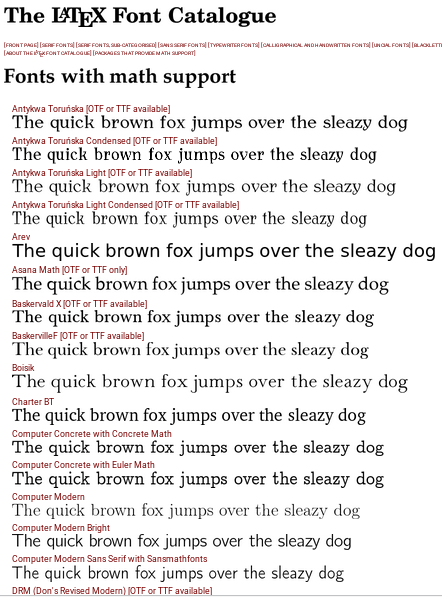
\includegraphics[height=.9\textheight]{fontcatalogue}

\end{columns}

  
\end{frame}

\section{Floats}




\subsection{Illustrating your document}



\begin{frame}[containsverbatim]
 \frametitle{Figures}
  


\begin{itemize}
  \item Figures and tables are inserted in the text as \emph{floats}
\begin{itemize}
  \item so called because they are not part of the text flux, but are instead positioned as if hovering over the page
  \item do not forget to include \lstinline!\usepackage{graphicx}! in the preamble if you plan to use figures!
\end{itemize}
\end{itemize}

\begin{LTXexample}
\begin{figure} % it's an environment!
\centering

\includegraphics[width=.9\textwidth]{comic1.png}
\caption{Taken from \url{http://phdcomics.com}}
\label{fig:comics}
\end{figure}
\end{LTXexample}

\begin{itemize}
  \item \emph{Note:} \verb!\label! is just a name you give to the float.
\begin{itemize}
  \item you can use it to reference it in the text, as we'll see shortly
\end{itemize}
\end{itemize}

\begin{itemize}
  \item you can also use \verb!\begin{figure}[htbp]!, where \texttt{h} (here), \texttt{t} (top), \texttt{b} (bottom) and \texttt{p} (page) are indications to where \LaTeX{} should place your float (it will only follow your suggestion if and when it is possible)
\begin{itemize}
  \item you can omit any of the \texttt{htbp} letters, or even change their order
\end{itemize}
\end{itemize}

\begin{itemize}
  \item Notice the command \lstinline!\url{webaddress}! to format a clickable link to a webpage. You need to put \lstinline!\usepackage{url}! in the preamble to use this feature
\end{itemize}

  
\end{frame}
\begin{frame}[containsverbatim]
 \frametitle{Tabular material}
  


\begin{itemize}
  \item Table floats are set in a \texttt{table} environment
  \item The \texttt{tabular} environment is used to typeset a table
\end{itemize}

\begin{LTXexample}
\begin{table}
\caption{List of equipments and suppliers}
\label{tab:dados}
\centering
\begin{tabular}{lcccc}
\hline
Equipment & Year & Vendor & PIC & Location \\
\hline
MO & 2015 & Zeiss & Joe & A5\\
MEV & 2012 & Hitachi & Moe & B3\\
XRD & 2014 & Panalytical & Larry & A2\\
\hline
\end{tabular}
\end{table}
\end{LTXexample}

\begin{itemize}
  \item Notice again the  use of \verb!\label! to tag the table float
  \item The \texttt{[htbp]} options are also available for tables
\end{itemize}

  
\end{frame}

\section{Math}




\subsection{The strongest card in the \LaTeX{} pack}



\begin{frame}[containsverbatim]
 \frametitle{Inline and display math}
  


\small

\begin{itemize}
  \item There are inline (using \$ \$) and displayed formulas (with the \texttt{equation} environment):
\end{itemize}

\begin{LTXexample}[preset=\let\label\orilabel]
A sphere of radius $R$ has a volume $V$ given by
\begin{equation}
V = \int_{0}^{2\pi} \int_{0}^{\pi} \int_{0}^{R} \rho^2 \sin \theta d\rho d\theta d\phi
= \frac{4}{3} \pi R^3 \,.
\label{eq:vol}
\end{equation}
It is not difficult to evaluate the integral, if you know what to do.
\end{LTXexample}

\begin{LTXexample}[preset=\let\label\orilabel]
The sum of the first $n$ terms of an arithmetic progression is
\begin{equation}
S_{n} = \sum_{i=1}^{n} a_{i} = \frac{(a_{1}+a_{n})n}{2} \,,
\end{equation}
in which $a_{i}=a_{i-1} + (n-1) r$ (valid for $2 \le i \le n$, with $a_{1}$ and $r$ given constants). Legend has it that Gauss discovered this formula while still a schoolboy\ldots
\end{LTXexample}

  
\end{frame}
\begin{frame}[containsverbatim]
 \frametitle{Some more options}
  


\begin{itemize}
  \item If you don't want to number a displayed equation, use \verb!\[ \]!, instead of the \texttt{equation} environment
\end{itemize}

\begin{LTXexample}[preset=\let\label\orilabel]
The sum of the first $n$ terms of an arithmetic progression is given by
\[
S_{n} = \sum_{i=1}^{n} a_{i} = \frac{(a_{1}+a_{n})n}{2} \,,
\]
in which $a_{i}=a_{i-1} + (n-1) r$ (valid for $2 \le i \le n$, with $a_{1}$ and $r$ given constants). Legend has it that Gauss discovered this formula while still a schoolboy\ldots
\end{LTXexample}

\begin{itemize}
  \item The \texttt{amsmath} package (as always, in the preamble) gives you access to lots of new math-related stuff
\end{itemize}

  
\end{frame}

\section{Cross-references}




\subsection{Referencing internally}



\begin{frame}[containsverbatim]
 \frametitle{The \texttt{$\backslash$label} --- \texttt{$\backslash$ref} system}
  


\begin{LTXexample}[preset=\let\label\orilabel]
\begin{figure}
\centering

\includegraphics[width=.6\textwidth]{comic-strip.jpg}
\caption{Taken from \url{http://phdcomics.com}.}
\label{fig:comic}
\end{figure}
\end{LTXexample}

\begin{LTXexample}
The situation we see depicted in Figure \ref{fig:comic} happens quite often in some cases\ldots
\end{LTXexample}

\begin{LTXexample}[preset=\let\label\orilabel]
\begin{equation}
e^{i \pi}  = -1
\label{eq:euler}
\end{equation}

Equation (\ref{eq:euler}) was first derived by Euler.
\end{LTXexample}

\begin{itemize}
  \item The \texttt{fig:}, \texttt{tab:} or \texttt{eq:} prefixes are not mandatory, but they are helpful to differentiate among the several kinds of stuff a label can point to (chapter, section, subsection, equation, list item, figure, table, etc., etc., etc.)
  \item The \verb!\pageref{lab}! command gives you the page in which \verb!\label{lab}! is found
\end{itemize}

  
\end{frame}

\section{Citations}




\subsection{Render unto C{\ae}sar --- Referencing externally}



\begin{frame}
 \frametitle{Reference managers}
  


\begin{itemize}
  \item I strongly recommend you use a reference manager to keep track of your bibliography. Below are two excellent choices that work virtually in any operating system
\end{itemize}

\begin{block}{Selected reference managers:}

\begin{itemize}
  \item JabRef --- \url{http://www.jabref.org} \\ 
\includegraphics[height=15mm]{jabref}
  \item Mendeley --- \url{https://www.mendeley.com} \\ 
\includegraphics[height=20mm]{mendeley}
\end{itemize}

\end{block}

  
\end{frame}
\begin{frame}[containsverbatim]
 \frametitle{How to use Bib\TeX}
  


\begin{itemize}
  \item The most widespread citation tool for \LaTeX{} is Bib\TeX{} (\url{http://www.bibtex.org})
  \item all your bibliographical references should be in (one or more) \texttt{bib} files
\end{itemize}

Put the following commands where you want your list of references to appear:
\begin{lstlisting}
\bibliography{mybibfile}
\bibliographystyle{plain} % there are dozens of styles to chose from
\end{lstlisting}

\begin{itemize}
  \item Then Bib\TeX{} does all the formatting work for you!
\end{itemize}

  
\end{frame}
\begin{frame}[containsverbatim]
 \frametitle{A Bib\TeX{} example}
  


% \footnotesize

\centering

\begin{columns}
\column{.5\textwidth}
\begin{itemize}
  \item For instance, let's say a file called \texttt{mybibfile.bib} constains the following entry (among others):
\end{itemize}

\begin{lstlisting}
@article{ferreira2018,
	author = {Ferreira, P. P. and Santos, F. B. and Machado, A. J. S. and Petrilli, H. M. and Eleno, L. T. F.},
	journal = {Phys. Rev. B},
	pages = {045126},
	title = {Insights into the unconventional superconductivity in {HfV$\textcolor{2$Ga$}{4$} and {ScV$}2$Ga$_4$} from first-principles electronic-structure calculations},
	volume = {98},
	year = {2018}
}
\end{lstlisting}

\column{.5\textwidth}

\begin{itemize}
  \item You can cite it in your work with the \verb!\cite! command:
\end{itemize}

\begin{lstlisting}
\documentclass[11pt]{article}

\begin{document}

Ferreira et al. \cite{ferreira2018} have shown that\ldots

\bibliography{mybibfile}
\bibliographystyle{plain}

\end{document}
\end{lstlisting}

\begin{framed}
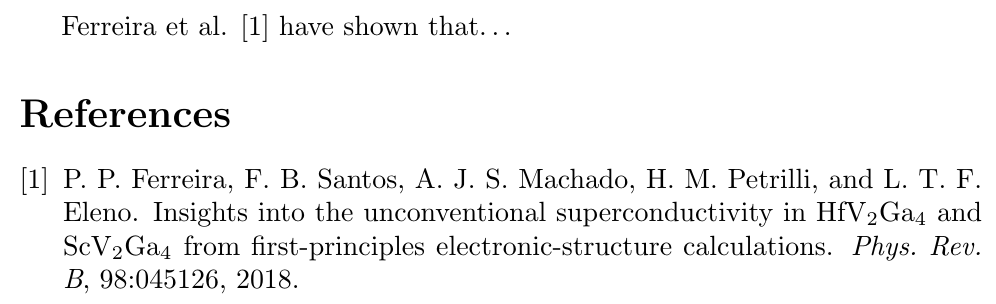
\includegraphics[height=.2\textheight]{referencia}
\end{framed}

\end{columns}


  
\end{frame}

\section[ABN\TeX2]{The ABN\TeX2 package}




\subsection{If there's no way around\ldots}



\begin{frame}
 \frametitle{ABN\TeX2 --- ABsurd Norms for \LaTeX}
  


\centering

\begin{itemize}
  \item Info only relevant to people working/studying in Brazil, mainly universities or research institutes
\end{itemize}


\includegraphics[height=20mm]{abntex}\\
\url{https://www.abntex.net.br}

\begin{itemize}
  \item ABN\TeX2 will take care of all weird formatting required by ABNT (Brazilian Bureau of Standards)
  \item on their website (link above) you'll find templates and tutorials
\end{itemize}

  
\end{frame}

\section{Envoi}




\subsection{Thank you for the music}



\begin{frame}
 \frametitle{Acknowledgements}
  

\framesubtitle{Thank you for your attention!}

\begin{center}

{\Huge \textcolor{red!80!black}{ \LaTeX{} is fun. } }


\vspace{ 8mm }


Find more help on:\\[2mm]
\begin{tabular}{ccc}

\includegraphics[height=20mm]{stackoverflow} &

\includegraphics[height=20mm]{ctan} &

\includegraphics[height=20mm]{latexproject}\\
\url{https://stackoverflow.com} &
\url{https://ctan.org} &
\url{https://www.latex-project.org}
\end{tabular}


\vspace{ 8mm }


Acknowledgements:\\[2mm]
\begin{tabular}{ccc}

\includegraphics[height=10mm]{usp} &

\includegraphics[height=12mm]{EEL-logo} &

\includegraphics[height=12mm]{ppgem} \\
\url{http://www5.usp.br} &
\url{http://site.eel.usp.br} &
\url{http://www.ppgem.eel.usp.br}
\end{tabular}


\vspace{ 6mm }


{Questions, corrections, comments and suggestions: \textcolor{blue}{ \href{mailto:luizeleno@usp.br}{luizeleno@usp.br} } \\
\url{http://www.demar.eel.usp.br/en/docentes/luiz-tadeu-fernandes-eleno.html}}


\vspace{ 3mm }


{\scriptsize This is version 1.1 of the tutorial. It can be freely distributed, but please point to the original project on github: \url{https://github.com/luizeleno/LaTeX-tutorial-for-newbies}}
\end{center}

  
\end{frame}


\end{document}

